\chapter{Wprowadzenie}
Głównym celem pracy jest opracowanie funkcjonalnego oprogramowania dedykowanego dla robota modularnego. By osiągnąć taki rezultat należało: zdefiniować oraz zaimplementować komunikację wewnętrzną i zewnętrzną, obsłużyć peryferia, wdrożyć mechanizmy pozwalające na diagnostykę i~serwisowanie urządzenia. W zakresie pracy mieściło się również dobranie komponentów elektronicznych, w tym serca układu -- mikroprocesora.

\section{Idea robota modularnego}
Od początku lat dwutysięcznych obserwuje się rozwój nowej dziedziny -- robotyki modularnej. Na~chwilę obecną należy zaliczyć ją do niszowych specjalizacji z zakresu robotyki, jednak zaczyna ona  zyskiwać na popularności \cite{state_art}. W momencie pisania pracy nie istnieje ogólnoprzyjęta definicja robota modularnego, jednak źródła zazwyczaj są zgodne co do charakterystyki urządzeń. Roboty muszą składać się z modułów: posiadających niezależne aktuatory oraz zdolnych do łączenia się i~rekonfiguracji \cite{modular_robots_theory, liu2009, state_art}. Każdy z członów traktowany jest jako niezależny w pełni funkcjonalny system, co wymusza pośrednio optymalizację konstrukcji mechanicznej oraz układów elektronicznych na poziomie pojedynczego segmentu. Inherentna zdolność tworzenia dowolnych topologii poprzez różne sposoby łączeń modułów sprawia, że roboty modularne mają lepsze zdolności adaptacyjne oraz wyższą niezawodność w stosunku do klasycznych robotów \cite{state_art, yoshida2003, liu2009}. Charakter urządzeń sprawia, że~nadają się one do dowolnych środowisk cechujących się dużą zmiennością.

\section{Istniejące roboty modularne i ich zastosowania}
W przeszłości powstało kilka urządzeń, które można zaliczyć do kategorii prototypów (ang. \textit{proof of concept}). Nie posiadają one konkretnych aplikacji i służą bardziej do badania możliwości i~praktyczności robotów modularnych. Jednym z pierwszych przykładów takiego robota jest M-TRAN II \cite{mtran}. Była to stosunkowo niewielka konstrukcja o kształcie przypominającym złożenie sześcianu oraz cylindra (rysunek \ref{fig: mtran}). Umożliwiała dynamiczne łączenie się członów z wykorzystaniem magnesów. Moduły mogły być łączone w dowolne topologie, w tym takie umożliwiające ruch przypominający wicie się. Głównym tematem eksplorowanym przez badaczy była tematyka rekonfiguracji -- zarówno pod względem fizycznym jak i procesu planowania kształtów robota. 

\begin{figure}[ht!]
    \centering
    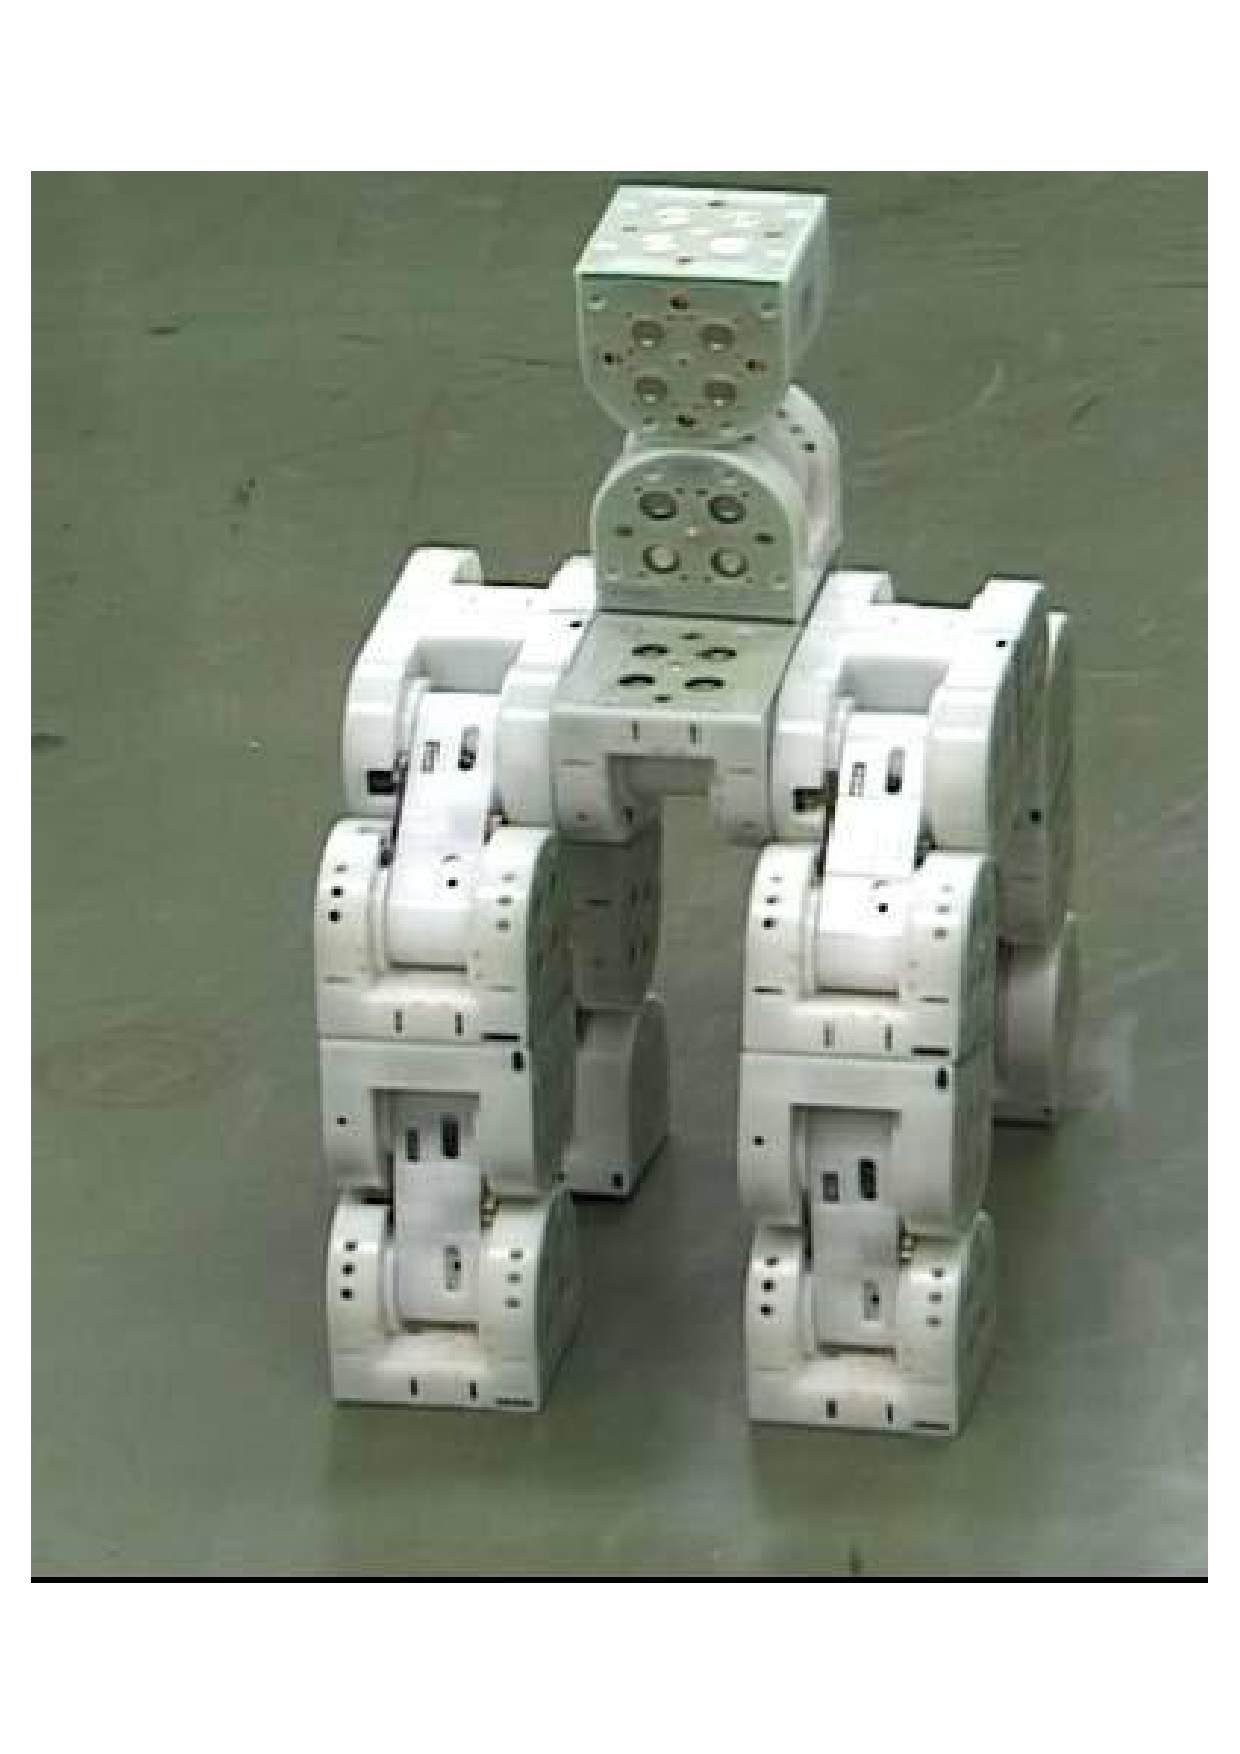
\includegraphics[width=0.5\textwidth]{rysunki/robots/mtran.pdf}
    \caption{\label{fig: mtran}Robot M-TRAN II \cite{mtran}}
\end{figure} 

Innym ciekawym projektem był robot Orimo \cite{chen2024}, który jest skrzyżowaniem się dziedzin robotyki modularnej oraz robotyki miękkiej (ang. \textit{soft robotics}). Jego koła zostały wykonane z kartonu oraz złożone techniką origami (rysunek \ref{fig: orimo}). Dzięki temu urządzenie jest w stanie zmienić swój kształt umożliwiając dwa sposoby lokomocji -- kroczenie oraz jeżdżenie. Robot miał być odpowiedzią na~problem znalezienia uniwersalnej metody poruszania się robotów.

\clearpage

\begin{figure}[ht!]
    \centering
    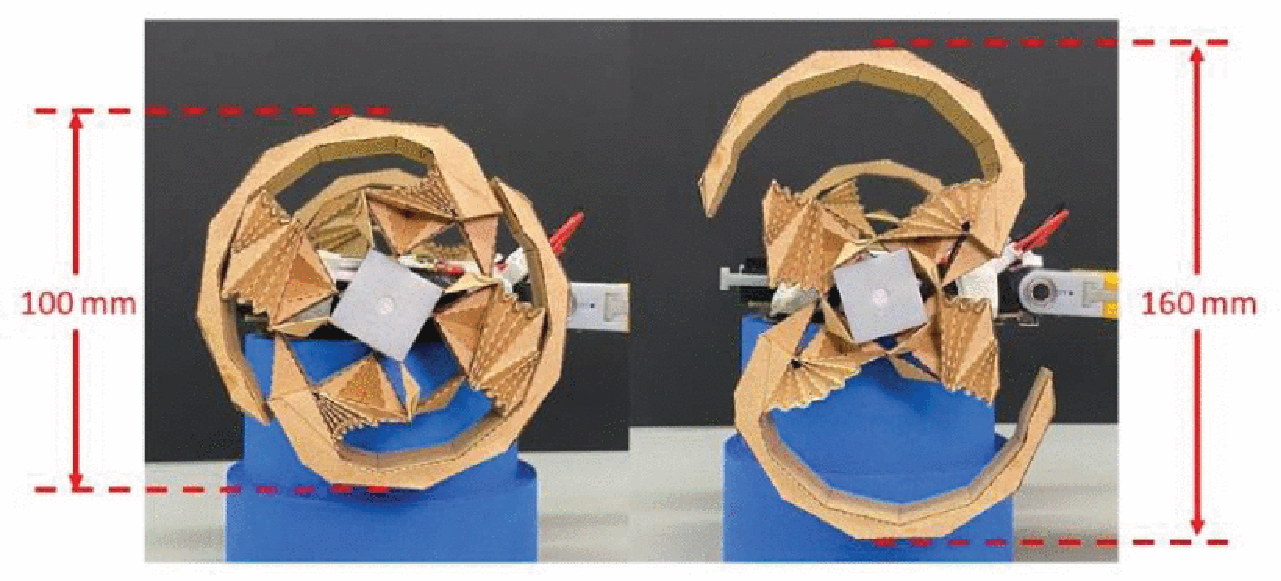
\includegraphics[width=0.7\textwidth]{rysunki/robots/orimo.pdf}
        \caption{\label{fig: orimo}Robot Orimo \cite{chen2024}}
\end{figure} 

W literaturze można znaleźć również bardziej użytkowe koncepcje wykorzystania robotów modularnych. Zaczynając od sektora edukacyjnego, gdzie uniwersalność oraz małe koszta sprawiają, że urządzenia tego typu są idealnym narzędziem do nauki. Przykładem takiej konstrukcji jest robot \textit{NEURobot} \cite{fang2009}, który w swoim założeniu ma wspierać nauczenie z zakresu teorii sterowania. Autorzy zapewnili możliwość sterowania urządzeniem z poziomu aplikacji \textit{Matlab}, co pozwala na~implementację złożonych algorytmów. Dodatkowo udostępniono narzędzie symulujące zachowanie cyfrowego bliźniaka. Konstrukcja robota oraz jego przykładowe topologie widoczne są na rysunku \ref{fig: neurobot}.

\begin{figure}[ht!]
    \centering
    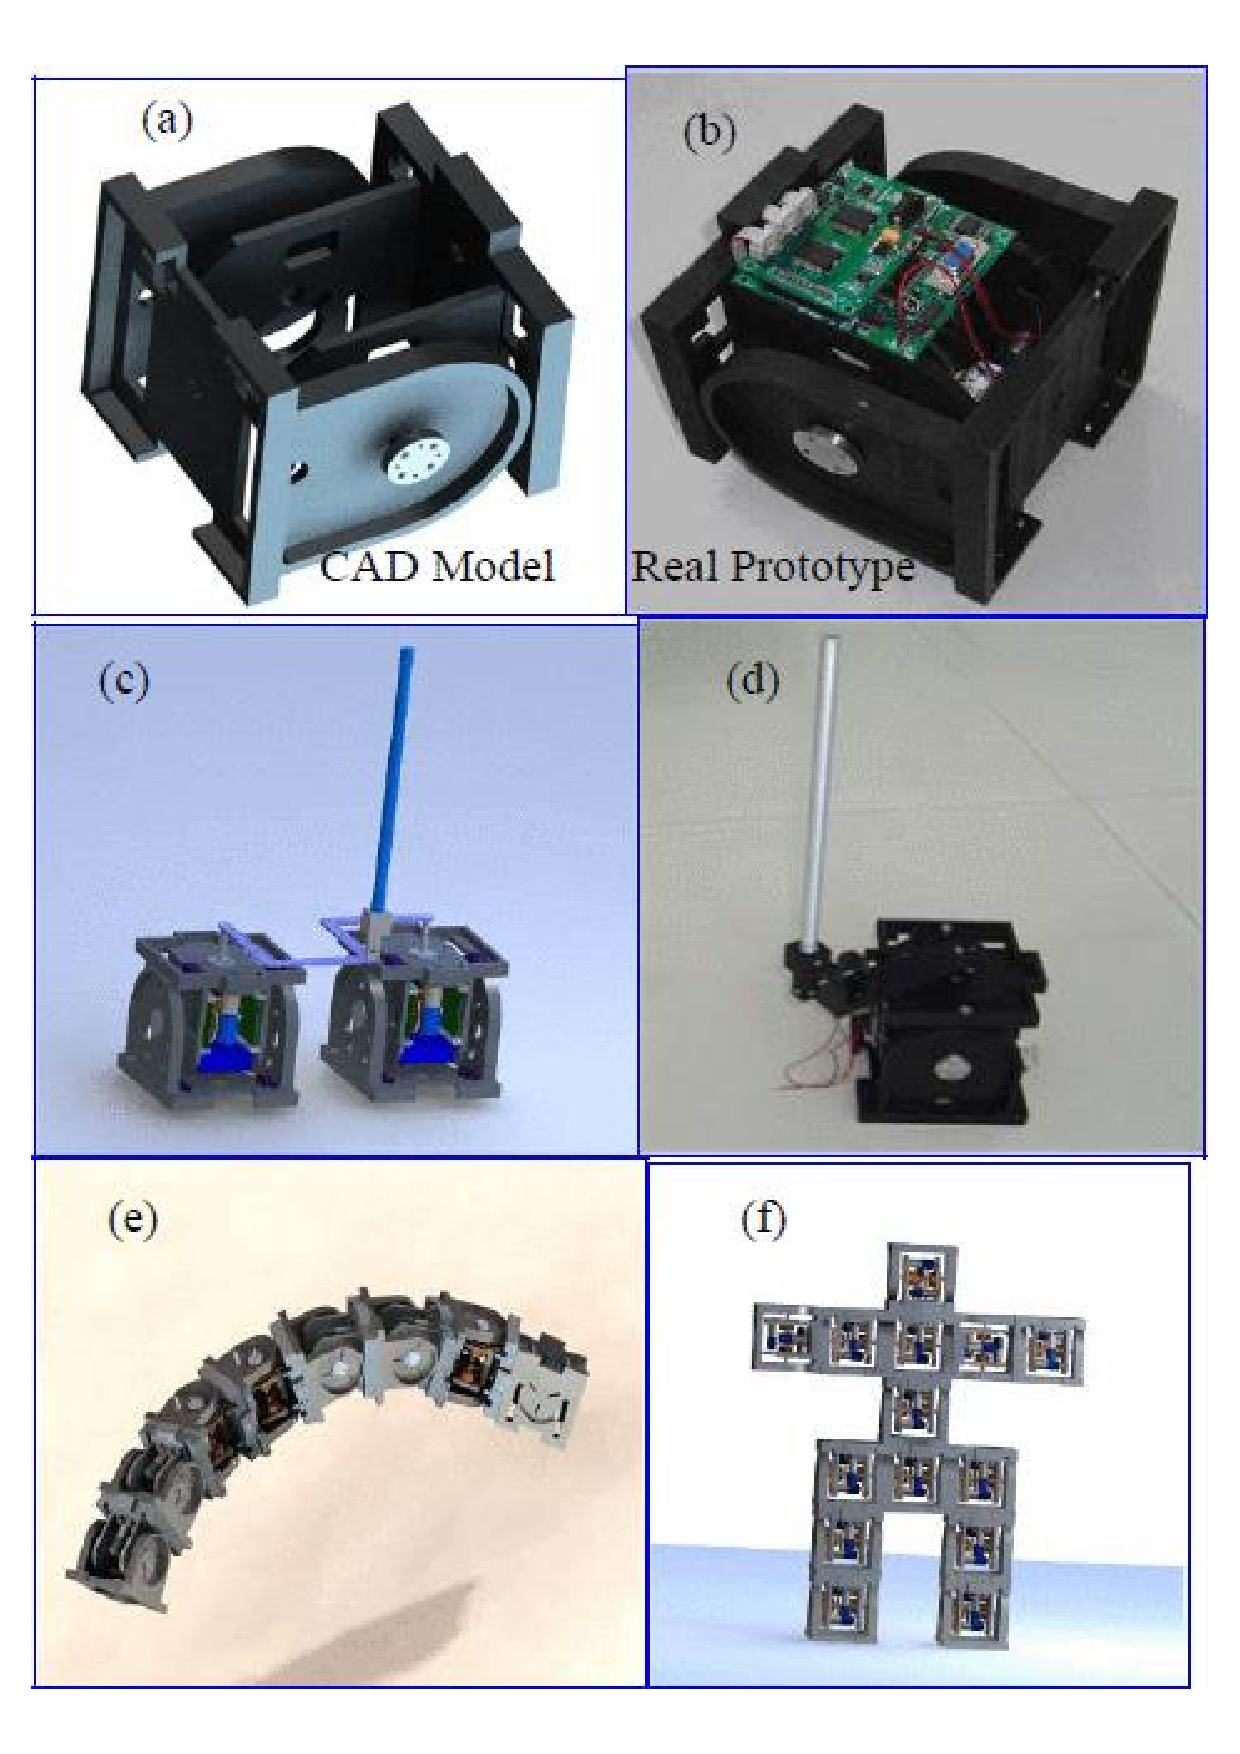
\includegraphics[width=0.4\textwidth]{rysunki/robots/neurobot.pdf}
    \caption{\label{fig: neurobot}Robot NEURobot \cite{fang2009}}
\end{figure} 

Przemysł kosmiczny jest kolejną branżą, której charakterystyka sprzyja robotom modularnym. Projektem wyspecjalizowanym i dostosowanym do tej aplikacji jest robot \textit{WORMS} stworzony w ramach programu \textit{2022 NASA BIG Idea Challenge} \cite{lordos2023}. Twórcy zakładają istnienie trzech generacji urządzeń, każda kolejna o bardziej złożonej konstrukcji oraz wyposażona w większą ilość czujników. W ramach pokazu możliwości stworzono sześcionożnego robota kroczącego (rysunek \ref{fig: worms}). Przeprowadzono również teoretyczną analizę czterech topologii, eksplorując ich zastosowania oraz właściwości (skalowalność, wytrzymałość etc.).

\begin{figure}[ht!]
    \centering
    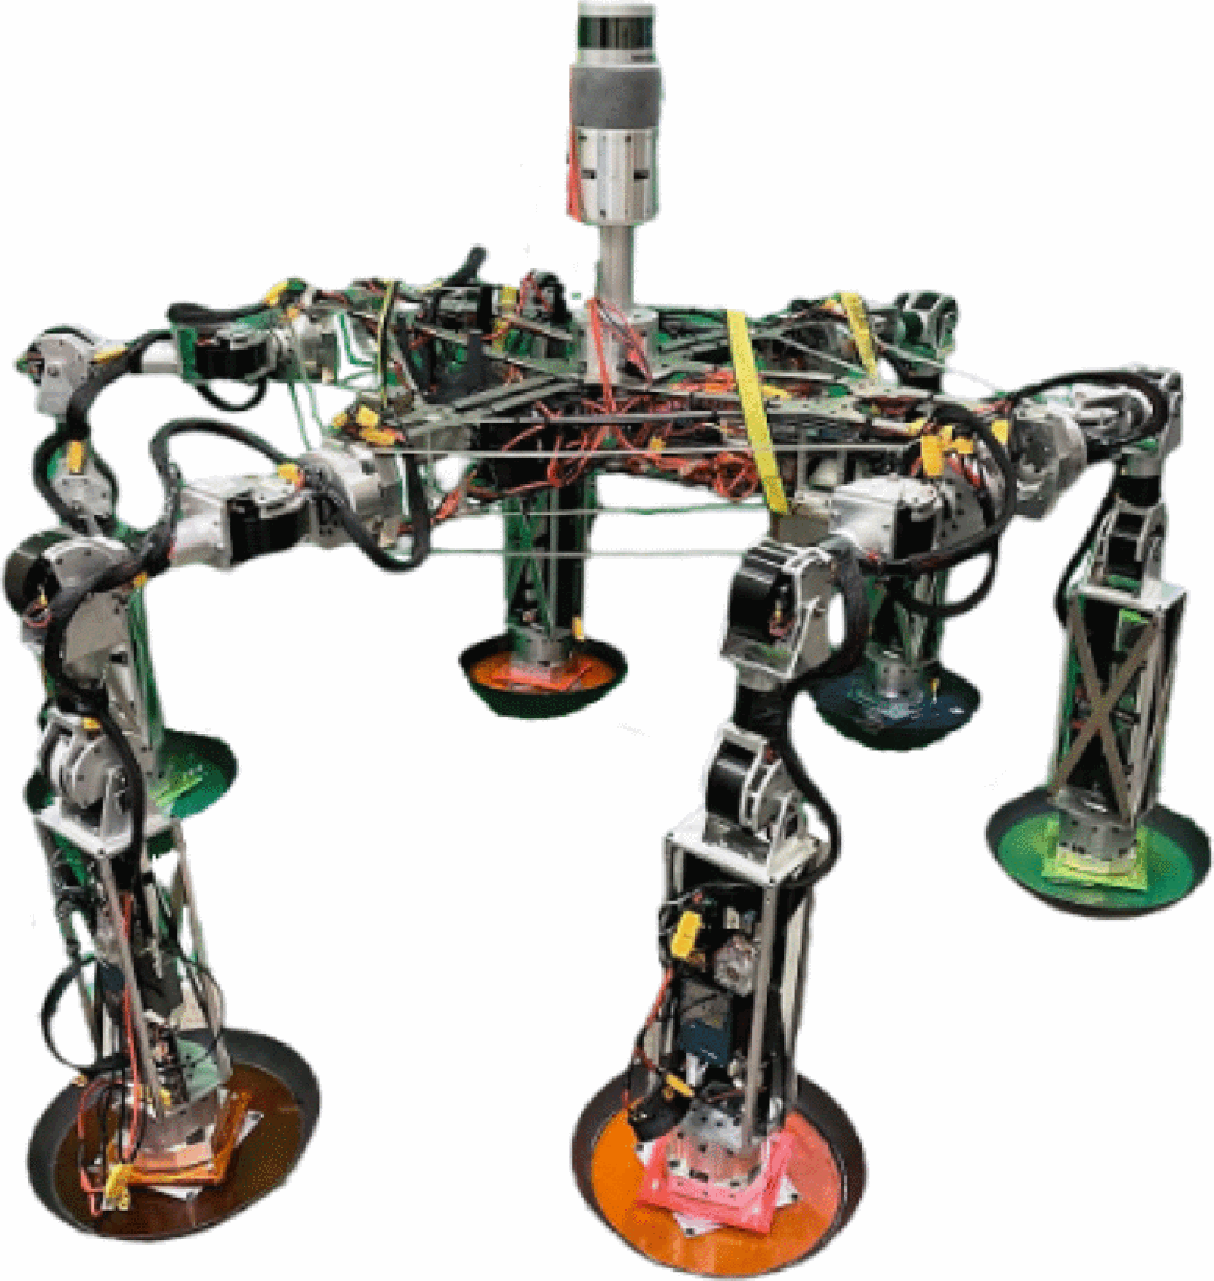
\includegraphics[width=0.5\textwidth]{rysunki/robots/worms.pdf}
    \caption{\label{fig: worms}Robot WORMS \cite{lordos2023}}
\end{figure} 

\subsection{Zestawienie robotów}
Na podstawie wcześniej przytoczonej literatury widoczne jest, że roboty modularne są bardzo zróżnicowane pod względem ich budowy mechanicznej, ale również ich zastosowań. W tabeli \ref{tab: comp_robots} zestawiono cechy robotów kluczowe dla tej pracy.
\begin{table}[!ht]
    \centering
    \begin{tabular}{p{2cm} ||p{2.5cm}|p{2.5cm}|p{3cm}|p{3cm}}
             & Orimo (2024) & WORMS (2022) & NEURobot (2009) & M-TRAN II (2003) \\ \hline \hline
            MCU & ESP32 S3 Wroom & Raspberry PI & TMS320F2812DSP & TMPN3120FE5M, PIC16F873/877 \\ \hline
            Komunikacja zewnętrzna & Wifi & Wifi & RF & LON \\ \hline
            Komunikacja wewnętrzna & Brak/Wifi & Obecna, niezdefiniowana & Brak/RF & Asynchroniczna szeregowa \\ \hline
            Sensory położenia & IMU, enkodery & --  & Enkodery & Akcelerometr \\ \hline
            Dodatkowe perfyferia & czujnik prądu & LIDAR & czujnik IR & -- \\ \hline
        \end{tabular}
    \caption{Zestawienie wybranych cech robotów modularnych}
    \label{tab: comp_robots}
\end{table}

Chociaż definitywne i dokładniejsze określenie cech wspólnych właściwych dla robotów modularnych wymagałoby przeanalizowanie większej ilości artykułów, przytoczone projekty mogą pozwolić na wyciągniecie kilku wniosków. 

Wspólnym mianownikiem okazuje się faworyzowanie komunikacji bezprzewodowej w przypadku komunikacji zewnętrznej (panel sterowniczy-robot). Prawdopodobnie wynika to z wygody takiego rozwiązania -- nie trzeba martwić się o prowadzenie przewodów łączeniowych a także urządzenie sterujące nie musi być wyposażone w specjalny interfejs (jak w przypadku Wifi). Kolejną własnością łączącą roboty jest fakt wyznaczania swojej pozycji na podstawie pomiarów otrzymywanych z~akcelerometrów i/lub enkoderów.

To co znacznie różni roboty między sobą to dobór mikrokontrolerów \gls{mcu} oraz dodatkowych peryferiów. Autorzy projektów nie podejmują się polemiki na temat ich doboru. W przypadku komponentów elektronicznych można zauważyć trend dostosowywania robota do konkretnej aplikacji. W przypadku robota \textit{WORMS} do konstrukcji dodano \gls{lidar}, który umożliwia implementację bardziej złożonych algorytmów lokalizacji i nawigacji -- są one potrzebne by urządzenie mogło pracować w nieznanym środowisku takim jak Księżyc. W projekcie \textit{NEURobot} autorzy uwzględnili możliwość złożenia z modułów robota mobilnego. W takiej aplikacji potrzebne są sensory zbliżeniowe, w tym przypadku czujniki podczerwieni \gls{ir}. Być może decyzja o wyborze konkretnych mikrokontrolerów była warunkowana głównie budową robota, jednak równie prawdopodobnymi powodami mogły być: preferencje programistów, dostępność na rynku oraz cena, obecność narzędzi/bibliotek dostosowanych do konkretnej rodziny mikrokontrolerów.

\section{Trudności w projektowaniu robotów modularnych}
Głównymi trudnościami związanymi z projektowaniem robotów modularnych są nie tylko kwestie mechaniczne takie jak wytrzymałość połączeń czy wielkość i waga modułów, ale również zagadnienie sterowania takimi układami o rozproszonej logice. Możliwe, że razem z rosnącym trendem zainteresowania tematyką sztucznej inteligencji zaobserwuje się rozwój i tej dziedziny. Standardowe podejście macierzowego opisu kinematyki robota bardzo szybko staje się niemożliwe do zrealizowania, dlatego dość popularną praktyką jest stosowanie algorytmów ewolucyjnych, nauczania ze wzmacnianiem czy sieci neuronowych \cite{hossein2015, }. 